\documentclass[12pt, a4paper]{article}
\usepackage[margin=1in]{geometry}
\setlength{\headheight}{13.6pt}
\addtolength{\topmargin}{-1.6pt}
\usepackage{graphicx}
\usepackage{float}
\usepackage{fancyhdr}
\usepackage{booktabs}
\usepackage{array}
\usepackage{longtable}
\usepackage{listings}
\usepackage{xcolor}
\usepackage{hyperref}
\usepackage{amsmath}
\usepackage{titlesec}
\usepackage{parskip}
\usepackage{pdfpages}

% ── Code listing style ───────────────────────────────────────
\definecolor{codebg}{RGB}{248,248,248}
\definecolor{codeframe}{RGB}{200,200,200}
\definecolor{sqlkw}{RGB}{0,0,180}
\definecolor{sqlstr}{RGB}{163,21,21}
\definecolor{sqlcmt}{RGB}{100,100,100}

\lstdefinestyle{sqlstyle}{
    backgroundcolor=\color{codebg},
    frame=single, rulecolor=\color{codeframe},
    basicstyle=\ttfamily\small,
    keywordstyle=\color{sqlkw}\bfseries,
    stringstyle=\color{sqlstr},
    commentstyle=\color{sqlcmt}\itshape,
    breaklines=true, breakatwhitespace=true,
    showstringspaces=false,
    morekeywords={CREATE,TABLE,PRIMARY,FOREIGN,KEY,REFERENCES,
                  INSERT,INTO,VALUES,SELECT,FROM,WHERE,JOIN,
                  GROUP,BY,ORDER,HAVING,NOT,NULL,DEFAULT,
                  PROCEDURE,FUNCTION,TRIGGER,BEGIN,END,
                  COMMIT,ROLLBACK,DECLARE,IF,THEN,ELSE,
                  SEQUENCE,CONSTRAINT,CHECK,UNIQUE,INDEX,
                  CURSOR,LOOP,FOR,WHEN,EXCEPTION,RAISE,
                  IN,OUT,NUMBER,VARCHAR2,DATE,RETURN,
                  AFTER,BEFORE,EACH,ROW,ON,NEXTVAL,AS,OR}
}
\lstset{style=sqlstyle}

% ── Page header ──────────────────────────────────────────────
\pagestyle{fancy}
\fancyhf{}
\lhead{\small Shopping Cart Management System}
\rhead{\small CSE-D | MIT Manipal}
\cfoot{\thepage}

% ── Title ────────────────────────────────────────────────────
\title{
    \vspace{-1cm}
    {\large Manipal Institute of Technology, Manipal} \\
    {\large Department of Computer Science and Engineering} \\[0.5cm]
    \rule{\linewidth}{0.5pt} \\[0.4cm]
    {\LARGE \textbf{Mini Project — Phase II}} \\[0.2cm]
    {\Large Implementing an Online Shopping Cart System} \\[0.2cm]
    \rule{\linewidth}{0.5pt}
}
\author{
    Udit Asthana \\ 240905310 \\ CSE-D
}
\date{February -- April 2026}
\begin{document}
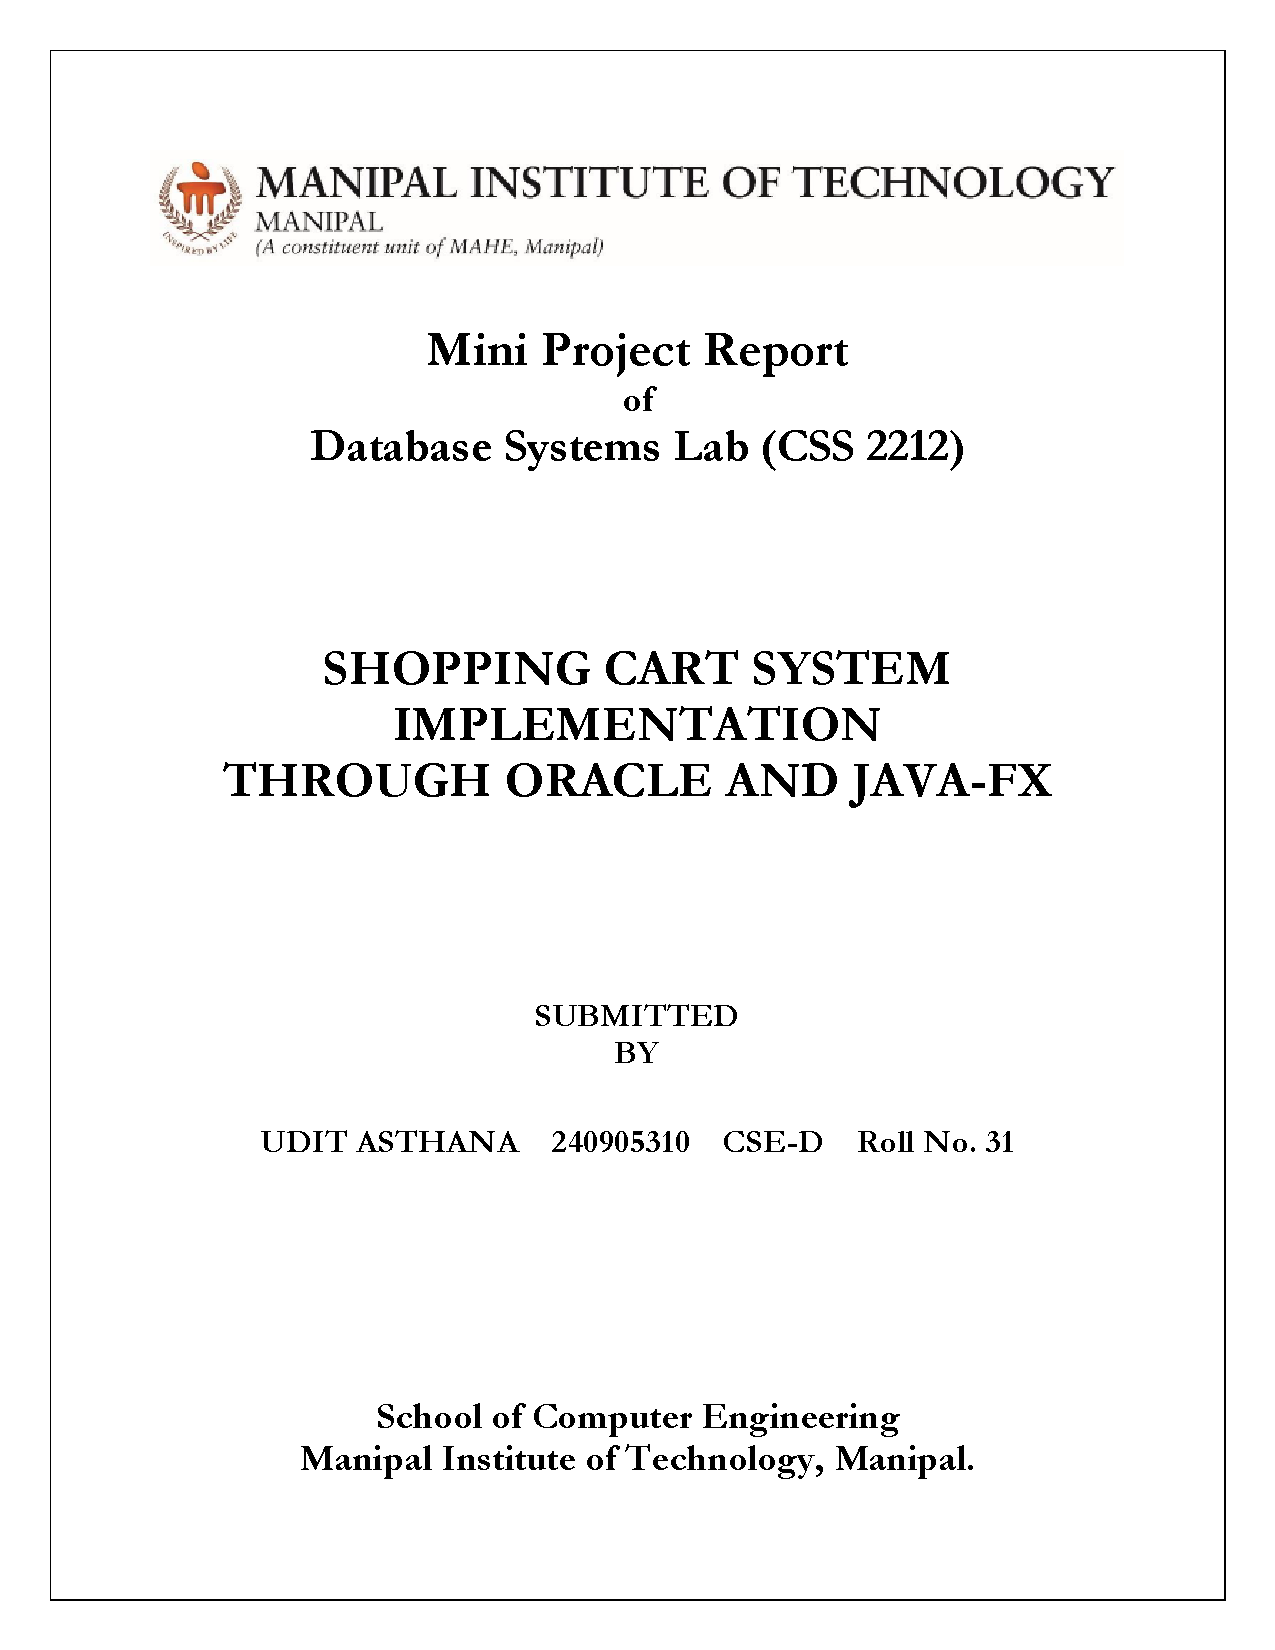
\includepdf[pages=1-3]{DBS Lab-Mini Project-Report Template.pdf}
\maketitle
\thispagestyle{fancy}
\tableofcontents
\newpage


\section{Abstract}

This project presents the design and implementation of a web-based Shopping Cart
Management System intended to demonstrate practical applications of Database Management
System (DBMS) concepts. The system enables users to browse items, add or remove products
from a virtual shopping cart, update quantities, and perform a consolidated checkout
operation. The primary focus is on database modelling, integrity enforcement, and
transaction management rather than building a full-scale commercial e-commerce platform.

The design extends the bookstore Entity--Relationship (E-R) schema of Exercise~6.21
(Silberschatz, \textit{Database System Concepts}, 7th ed.) to incorporate additional
entities such as \textit{Cart}, \textit{Order}, \textit{Inventory}, and \textit{Payment},
ensuring proper relationships, normalisation, and constraint enforcement. The relational
schema is implemented using Oracle 21c XE with primary keys, foreign keys, check
constraints, sequences, triggers, and stored procedures. A Java JDBC layer demonstrates
database connectivity and calls to PL/SQL procedures for cart operations, stock
verification, and atomic order placement.

\section{Introduction}

The rapid growth of e-commerce has made efficient shopping cart systems a
cornerstone of modern retail infrastructure. Managing product catalogues,
customer sessions, inventory, and atomic transactions demands a well-designed
relational database backend capable of enforcing integrity at every layer.

This project implements a Shopping Cart Management System for an online
bookstore, built atop Oracle 21c XE using JDBC and JavaFX. The system extends
the bookstore Entity--Relationship schema of Exercise 6.21 (Silberschatz,
\textit{Database System Concepts}, 7th ed.) to support a complete purchase
lifecycle: browsing, cart management, stock verification, and atomic checkout.

The primary objective is not to replicate a commercial platform but to
demonstrate rigorous application of DBMS principles --- normalisation,
constraint enforcement, stored procedures, triggers, and transaction
management --- within a working, interactive system.

\section{Problem Statement}
\subsection{Background}
Design and implement a shopping cart system that lets shoppers collect items into a
shopping cart and purchase them together. The system is built by extending the
bookstore E-R schema of \textbf{Exercise 6.21, Chapter 6} (Korth, 6th Edition).
Stock availability must be verified at checkout, and out-of-stock situations must be
handled gracefully.
\subsection{Data Requirements}
The system must maintain the following data:
\begin{itemize}
    \item \textbf{Books}: identified by ISBN; storing title, publication year, price,
          genre, author, and publisher.
    \item \textbf{Authors}: name, address, URL.
    \item \textbf{Publishers}: name, address, phone, URL.
    \item \textbf{Customers}: unique email, name, address, phone, hashed password,
          registration timestamp.
    \item \textbf{Warehouses}: code, address, phone.
    \item \textbf{Inventory}: per-warehouse stock count for each book.
    \item \textbf{Cart}: links a customer to a set of items; tracks status
          (ACTIVE, CHECKED\_OUT, ABANDONED).
    \item \textbf{Cart Items}: book + quantity within a cart.
    \item \textbf{Orders}: placed from a cart; captures total amount and order status.
    \item \textbf{Order Items}: snapshot of each book's price and quantity at order time.
    \item \textbf{Payments}: method, amount, and status for each order.
\end{itemize}

\subsection{Functional Requirements}
\begin{enumerate}
    \item Browse all available books with author/publisher details.
    \item Add, update quantity, and remove books from an active cart.
    \item Check total stock availability before and during checkout.
    \item Atomically place an order from a cart using a transaction; rollback on failure.
    \item Automatically decrement inventory on order placement (trigger).
    \item Mark a cart as CHECKED\_OUT when an order is placed (trigger).
    \item Prevent negative inventory at all times (trigger + constraint).
    \item Record payment alongside each order.
    \item Support complex reporting: revenue by publisher, demand forecasting,
          order receipts, and customer analytics.
\end{enumerate}


\section{Methodology}
\subsection{Development Approach}
The project followed an incremental design process: the database schema was
designed and normalised first, followed by DDL implementation, then PL/SQL
logic, and finally the Java JDBC frontend. Each layer was tested independently
before integration.

\subsection{Tools and Technologies}
\begin{itemize}
    \item \textbf{Database:} Oracle 21c XE (XEPDB1) for schema hosting,
          constraint enforcement, and PL/SQL execution.
    \item \textbf{Connectivity:} Oracle JDBC Type-4 thin driver
          (\texttt{ojdbc11.jar}) for Java--database communication.
    \item \textbf{Frontend:} JavaFX for the graphical user interface,
          providing a dark-themed tabbed dashboard.
    \item \textbf{Build Tool:} Apache Maven for dependency management
          and compilation.
    \item \textbf{IDE:} IntelliJ IDEA for development and debugging.
\end{itemize}

\subsection{Database Design Process}
The original Exercise 6.21 E-R schema was analysed to identify entities
relevant to a shopping cart context. Extensions were then designed to cover
the full purchase lifecycle, including Cart, Inventory, Orders, Order Items,
and Payment entities. Each table was verified against 3NF before DDL was
written.

\subsection{Implementation Sequence}
\begin{enumerate}
    \item Schema design and normalisation.
    \item DDL: table definitions, constraints, and sequences.
    \item Sample data insertion across all 11 tables.
    \item PL/SQL: functions, procedures, and triggers.
    \item JDBC layer: connection setup, query execution, and procedure calls.
    \item JavaFX UI: one tab per core operation, with a live console log.
    \item Testing against all scenarios in Table~5.
\end{enumerate}

\subsection{Transaction Strategy}
All multi-step write operations --- particularly checkout --- use manual
transaction control (\texttt{setAutoCommit(false)}) with explicit
\texttt{COMMIT} on success and \texttt{ROLLBACK} in the exception handler,
ensuring atomicity across order placement, inventory decrement, and payment
recording.

\section{E-R Diagram and Schema Extension}

\subsection{Original E-R Schema (Exercise 6.21)}

The original bookstore schema from Silberschatz et al.\ contains the following
entities and relationships:

\begin{itemize}
    \item \textbf{Entities}: \textit{author} (name, address, URL),
          \textit{book} (ISBN, title, year, price),
          \textit{publisher} (name, address, phone, URL),
          \textit{customer} (email, name, address, phone),
          \textit{shopping\_basket} (basket\_id),
          \textit{warehouse} (code, address, phone).
    \item \textbf{Relationships}: \textit{written\_by} (book--author),
          \textit{published\_by} (book--publisher),
          \textit{basket\_of} (basket--customer),
          \textit{contains} (basket--book, with attribute \textit{number}),
          \textit{stocks} (warehouse--book, with attribute \textit{number}).
\end{itemize}

\begin{figure}[H]
    \centering
    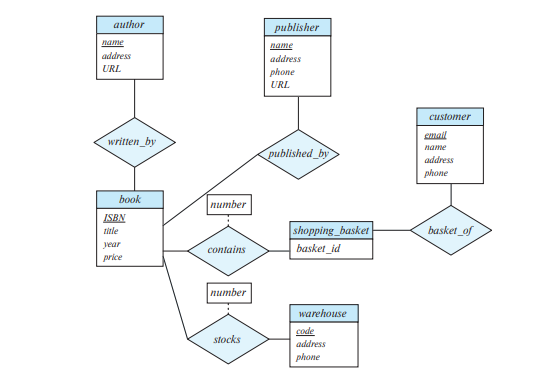
\includegraphics[width=0.75\linewidth]{image.png}
    \caption{Original E-R schema from Exercise 6.21 (Silberschatz et al.)}
    \label{fig:original-er}
\end{figure}

\subsection{Extensions Made}

Table~\ref{tab:extensions} summarises the extensions applied to the original schema.

\begin{table}[H]
\centering
\caption{Schema extensions beyond Exercise 6.21}
\label{tab:extensions}
\begin{tabular}{lll}
\toprule
\textbf{Original} & \textbf{Change} & \textbf{Reason} \\
\midrule
\textit{book}            & Added \textit{genre}, \textit{description} & Richer browsing \\
\textit{customer}        & Added \textit{password\_hash}, \textit{created\_at} & Auth + analytics \\
\textit{shopping\_basket} & Renamed to \textit{cart}; added \textit{status}, \textit{created\_at} & Lifecycle tracking \\
\textit{contains}        & Became \textit{CART\_ITEMS} table & Proper relation \\
\textit{stocks}          & Became \textit{INVENTORY} table & Warehouse tracking \\
---                      & New: \textit{ORDERS}            & Order management \\
---                      & New: \textit{ORDER\_ITEMS}      & Per-order snapshot \\
---                      & New: \textit{PAYMENT}           & Payment tracking \\
\bottomrule
\end{tabular}
\end{table}

\section{Relational Schema and Normalisation}

\subsection{Relational Tables}
\begin{align*}
&\textbf{AUTHOR}(\underline{name},\ address,\ url) \\
&\textbf{PUBLISHER}(\underline{name},\ address,\ phone,\ url) \\
&\textbf{BOOK}(\underline{isbn},\ title,\ year,\ price,\ genre,\ description,\ \underline{author\_name},\ \underline{publisher\_name}) \\
&\textbf{CUSTOMER}(\underline{cust\_id},\ email,\ name,\ address,\ phone,\ password\_hash,\ created\_at) \\
&\textbf{WAREHOUSE}(\underline{code},\ address,\ phone) \\
&\textbf{INVENTORY}(\underline{warehouse\_code},\ \underline{isbn},\ quantity) \\
&\textbf{CART}(\underline{cart\_id},\ \underline{cust\_id},\ status,\ created\_at,\ updated\_at) \\
&\textbf{CART\_ITEMS}(\underline{cart\_id},\ \underline{isbn},\ quantity) \\
&\textbf{ORDERS}(\underline{order\_id},\ \underline{cust\_id},\ \underline{cart\_id},\ order\_date,\ total\_amount,\ status) \\
&\textbf{ORDER\_ITEMS}(\underline{order\_id},\ \underline{isbn},\ quantity,\ price\_at\_order) \\
&\textbf{PAYMENT}(\underline{payment\_id},\ \underline{order\_id},\ amount,\ method,\ payment\_date,\ status)
\end{align*}
(Underlined attributes are primary keys; foreign key references follow from context.)


\subsection{Normalisation}

All tables satisfy \textbf{Third Normal Form (3NF)} / \textbf{BCNF}:

\begin{itemize}
    \item \textbf{1NF}: All attributes are atomic. No multi-valued columns.
    \item \textbf{2NF}: No partial dependencies exist. In \texttt{ORDER\_ITEMS}
          the non-key attribute \texttt{price\_at\_order} depends on the full
          composite key \{order\_id, isbn\}, not a subset.
    \item \textbf{3NF}: No transitive dependencies. \texttt{BOOK} stores
          \texttt{author\_name} and \texttt{publisher\_name} as FKs only —
          author details live entirely in \texttt{AUTHOR}.
\end{itemize}

A deliberate design choice: \texttt{ORDER\_ITEMS.price\_at\_order} snapshots the
book price at time of purchase. Although \texttt{BOOK.price} exists, this is not a
transitive dependency because the historical price is a distinct fact from the
current price.

\section{DDL — Table Definitions and Constraints}

The following listings show representative DDL. Full code is in
\texttt{schema\_setup.sql}.

\begin{lstlisting}[caption={BOOK and INVENTORY table definitions}]
CREATE TABLE BOOK (
    isbn           VARCHAR2(20)  NOT NULL,
    title          VARCHAR2(255) NOT NULL,
    year           NUMBER(4)     NOT NULL,
    price          NUMBER(8,2)   NOT NULL,
    genre          VARCHAR2(50),
    author_name    VARCHAR2(100) NOT NULL,
    publisher_name VARCHAR2(100) NOT NULL,
    CONSTRAINT pk_book        PRIMARY KEY (isbn),
    CONSTRAINT fk_book_author FOREIGN KEY (author_name)
                              REFERENCES AUTHOR(name),
    CONSTRAINT fk_book_pub    FOREIGN KEY (publisher_name)
                              REFERENCES PUBLISHER(name),
    CONSTRAINT chk_book_price CHECK (price > 0),
    CONSTRAINT chk_book_year  CHECK (year BETWEEN 1000 AND 2100)
);

CREATE TABLE INVENTORY (
    warehouse_code VARCHAR2(20) NOT NULL,
    isbn           VARCHAR2(20) NOT NULL,
    quantity       NUMBER(6)    DEFAULT 0 NOT NULL,
    CONSTRAINT pk_inventory     PRIMARY KEY (warehouse_code, isbn),
    CONSTRAINT fk_inv_warehouse FOREIGN KEY (warehouse_code)
                                REFERENCES WAREHOUSE(code),
    CONSTRAINT fk_inv_book      FOREIGN KEY (isbn)
                                REFERENCES BOOK(isbn),
    CONSTRAINT chk_inv_qty      CHECK (quantity >= 0)
);
\end{lstlisting}

\begin{lstlisting}[caption={CART and ORDERS with status constraints}]
CREATE TABLE CART (
    cart_id    NUMBER       DEFAULT SEQ_CART.NEXTVAL NOT NULL,
    cust_id    NUMBER       NOT NULL,
    status     VARCHAR2(20) DEFAULT 'ACTIVE' NOT NULL,
    created_at DATE         DEFAULT SYSDATE,
    CONSTRAINT pk_cart       PRIMARY KEY (cart_id),
    CONSTRAINT fk_cart_cust  FOREIGN KEY (cust_id)
                             REFERENCES CUSTOMER(cust_id),
    CONSTRAINT chk_cart_status
        CHECK (status IN ('ACTIVE','CHECKED_OUT','ABANDONED'))
);
\end{lstlisting}

\section{SQL Queries}

\subsection{Basic Queries}

\begin{lstlisting}[caption={Q1: All books with author and publisher}]
SELECT b.isbn, b.title, b.year, b.price,
       a.name AS author, p.name AS publisher
FROM   BOOK b
JOIN   AUTHOR    a ON a.name = b.author_name
JOIN   PUBLISHER p ON p.name = b.publisher_name
ORDER  BY b.title;
\end{lstlisting}

\begin{lstlisting}[caption={Q2: Active cart contents for a customer}]
SELECT b.title, b.price, ci.quantity,
       (b.price * ci.quantity) AS line_total
FROM   CART c
JOIN   CART_ITEMS ci ON ci.cart_id = c.cart_id
JOIN   BOOK b        ON b.isbn     = ci.isbn
WHERE  c.cust_id = 1 AND c.status = 'ACTIVE';
\end{lstlisting}

\begin{lstlisting}[caption={Q3: Total stock per book across all warehouses}]
SELECT b.title, SUM(i.quantity) AS total_stock
FROM   INVENTORY i
JOIN   BOOK b ON b.isbn = i.isbn
GROUP  BY b.title
ORDER  BY total_stock DESC;
\end{lstlisting}

\subsection{Complex Queries}

\begin{lstlisting}[caption={Q9: Stock availability check for cart items}]
SELECT  b.title,
        ci.quantity             AS qty_wanted,
        NVL(SUM(i.quantity),0)  AS total_available,
        CASE
            WHEN NVL(SUM(i.quantity),0) >= ci.quantity THEN 'IN STOCK'
            WHEN NVL(SUM(i.quantity),0) > 0            THEN 'PARTIAL'
            ELSE                                            'OUT OF STOCK'
        END AS availability
FROM    CART_ITEMS ci
JOIN    BOOK       b  ON b.isbn = ci.isbn
LEFT JOIN INVENTORY i ON i.isbn = ci.isbn
WHERE   ci.cart_id = 1
GROUP   BY b.title, ci.quantity;
\end{lstlisting}

\begin{lstlisting}[caption={Q8: Active cart summary with totals}]
SELECT  cu.name AS customer, c.cart_id,
        COUNT(ci.isbn)             AS distinct_titles,
        SUM(ci.quantity)           AS total_books,
        SUM(b.price * ci.quantity) AS cart_value
FROM    CART c
JOIN    CUSTOMER   cu ON cu.cust_id = c.cust_id
JOIN    CART_ITEMS ci ON ci.cart_id = c.cart_id
JOIN    BOOK       b  ON b.isbn     = ci.isbn
WHERE   c.status = 'ACTIVE'
GROUP   BY cu.name, c.cart_id
ORDER   BY cart_value DESC;
\end{lstlisting}

\begin{lstlisting}[caption={Q11: Revenue per publisher (complex aggregation)}]
SELECT  p.name AS publisher,
        COUNT(DISTINCT o.order_id)           AS total_orders,
        SUM(oi.quantity)                     AS books_sold,
        SUM(oi.price_at_order * oi.quantity) AS revenue
FROM    ORDER_ITEMS oi
JOIN    BOOK        b  ON b.isbn     = oi.isbn
JOIN    PUBLISHER   p  ON p.name     = b.publisher_name
JOIN    ORDERS      o  ON o.order_id = oi.order_id
WHERE   o.status IN ('PLACED','SHIPPED','DELIVERED')
GROUP   BY p.name
ORDER   BY revenue DESC;
\end{lstlisting}

\section{PL/SQL Procedures, Functions, and Triggers}

\subsection{Functions}

\begin{lstlisting}[caption={get\_total\_stock: total stock across all warehouses}]
CREATE OR REPLACE FUNCTION get_total_stock(p_isbn IN VARCHAR2)
RETURN NUMBER IS
    v_total NUMBER := 0;
BEGIN
    SELECT NVL(SUM(quantity), 0) INTO v_total
    FROM   INVENTORY WHERE isbn = p_isbn;
    RETURN v_total;
END get_total_stock;
\end{lstlisting}

\subsection{Procedures}

\begin{lstlisting}[caption={add\_to\_cart: add a book to a customer's active cart}]
CREATE OR REPLACE PROCEDURE add_to_cart(
    p_cust_id  IN NUMBER,
    p_isbn     IN VARCHAR2,
    p_quantity IN NUMBER DEFAULT 1
) AS
    v_cart_id NUMBER;
    v_stock   NUMBER;
BEGIN
    v_stock := get_total_stock(p_isbn);
    IF v_stock < p_quantity THEN
        RAISE_APPLICATION_ERROR(-20010,
            'Insufficient stock. Available: ' || v_stock);
    END IF;
    -- get or create active cart, then upsert cart item
    ...
    COMMIT;
END add_to_cart;
\end{lstlisting}


\begin{lstlisting}[caption={checkout: atomic order placement with rollback}]
CREATE OR REPLACE PROCEDURE checkout(
    p_cust_id        IN  NUMBER,
    p_payment_method IN  VARCHAR2,
    p_order_id       OUT NUMBER
) AS BEGIN
    -- 1. Validate cart not empty
    -- 2. Check all items in stock
    -- 3. INSERT into ORDERS
    -- 4. INSERT into ORDER_ITEMS  (triggers fire here)
    -- 5. INSERT into PAYMENT
    COMMIT;
EXCEPTION
    WHEN OTHERS THEN ROLLBACK; RAISE;
END checkout;
\end{lstlisting}

\subsection{Triggers}

\begin{table}[H]
\centering
\caption{Summary of triggers}
\begin{tabular}{lll}
\toprule
\textbf{Trigger} & \textbf{Event} & \textbf{Action} \\
\midrule
\texttt{trg\_decrement\_stock}    & AFTER INSERT on ORDER\_ITEMS & Decrement INVENTORY \\
\texttt{trg\_checkout\_cart}      & AFTER INSERT on ORDERS       & Mark cart CHECKED\_OUT \\
\texttt{trg\_cart\_updated}       & AFTER DML on CART\_ITEMS     & Update cart timestamp \\
\texttt{trg\_prevent\_neg\_stock} & BEFORE UPDATE on INVENTORY   & Reject negative qty \\
\texttt{trg\_lock\_checked\_out}  & BEFORE DML on CART\_ITEMS    & Reject non-ACTIVE cart \\
\bottomrule
\end{tabular}
\end{table}

\begin{lstlisting}[caption={trg\_decrement\_stock trigger}]
CREATE OR REPLACE TRIGGER trg_decrement_stock
AFTER INSERT ON ORDER_ITEMS
FOR EACH ROW
BEGIN
    UPDATE INVENTORY
    SET    quantity = quantity - :NEW.quantity
    WHERE  isbn = :NEW.isbn;
END;
\end{lstlisting}


\section{Java DB Connectivity}


The file \texttt{ShoppingCartDB.java} demonstrates Oracle JDBC connectivity
using the Type-4 thin driver (\texttt{ojdbc11.jar}).

\begin{lstlisting}[language=Java, caption={JDBC connection setup}]
private static final String URL =
    "jdbc:oracle:thin:@localhost:1521/XEPDB1";

public static Connection getConnection() throws SQLException {
    return DriverManager.getConnection(URL, USER, PASSWORD);
}
\end{lstlisting}

\begin{lstlisting}[language=Java, caption={Calling the checkout PL/SQL procedure}]
String sql = "BEGIN checkout(?, ?, ?); END;";
CallableStatement cs = con.prepareCall(sql);
cs.setInt(1, custId);
cs.setString(2, paymentMethod);
cs.registerOutParameter(3, Types.NUMERIC); // OUT p_order_id
cs.execute();
int orderId = cs.getInt(3);
\end{lstlisting}

Key JDBC patterns demonstrated:
\begin{itemize}
    \item \texttt{Statement} for simple SELECT queries.
    \item \texttt{PreparedStatement} for parameterised queries (prevents SQL injection).
    \item \texttt{CallableStatement} for PL/SQL procedure and function calls.
    \item Manual \texttt{con.setAutoCommit(false)} with explicit \texttt{COMMIT}/\texttt{ROLLBACK}.
\end{itemize}


\section{Transaction Management}


The checkout operation is the most critical transaction in the system. It follows an
all-or-nothing strategy:

\begin{enumerate}
    \item Validate that the cart contains at least one item.
    \item For every cart item, verify that total warehouse stock $\geq$ quantity
          requested. If any item fails, raise an error before any \texttt{INSERT}.
    \item Insert one row into \texttt{ORDERS}.
    \item Insert rows into \texttt{ORDER\_ITEMS}; triggers fire automatically to
          decrement \texttt{INVENTORY} and mark the cart \texttt{CHECKED\_OUT}.
    \item Insert one row into \texttt{PAYMENT}.
    \item \texttt{COMMIT} — all five steps succeed atomically.
    \item \texttt{ROLLBACK} in the \texttt{WHEN OTHERS} exception handler if any step fails.
\end{enumerate}

This guarantees that partial orders (e.g., payment recorded but inventory not
decremented) can never occur.


\section{Sample Data}


\begin{table}[H]
\centering
\caption{Sample books in the system}
\begin{tabular}{llrr}
\toprule
\textbf{ISBN} & \textbf{Title} & \textbf{Year} & \textbf{Price (Rs.)} \\
\midrule
978-0-07-352332-3 & Database System Concepts & 2019 & 899 \\
978-0-13-468599-1 & Operating System Concepts & 2018 & 799 \\
978-0-13-235088-4 & Clean Code & 2008 & 649 \\
978-0-13-212227-1 & Computer Networks & 2021 & 749 \\
978-0-06-231609-7 & Sapiens & 2015 & 499 \\
978-0-06-244558-9 & Homo Deus & 2017 & 549 \\
\bottomrule
\end{tabular}
\end{table}

\begin{table}[H]
\centering
\caption{Warehouses and total inventory}
\begin{tabular}{lll}
\toprule
\textbf{Code} & \textbf{Location} & \textbf{Books Stocked} \\
\midrule
WH-MUM & Andheri East, Mumbai     & 3 titles \\
WH-BLR & Whitefield, Bengaluru    & 3 titles \\
WH-DEL & Okhla Phase II, New Delhi & 3 titles \\
\bottomrule
\end{tabular}
\end{table}


\section{UI Design}


The application is built using \textbf{JavaFX} with a dark-themed dashboard
interface. It connects to Oracle 21c XE via JDBC and exposes all six core
operations as tabs. A persistent console panel at the bottom logs every DB
operation in real time, and a status indicator in the header confirms the
active Oracle connection (\texttt{● XEPDB1}).

\subsection{Books Listing}

\begin{figure}[H]
    \centering
    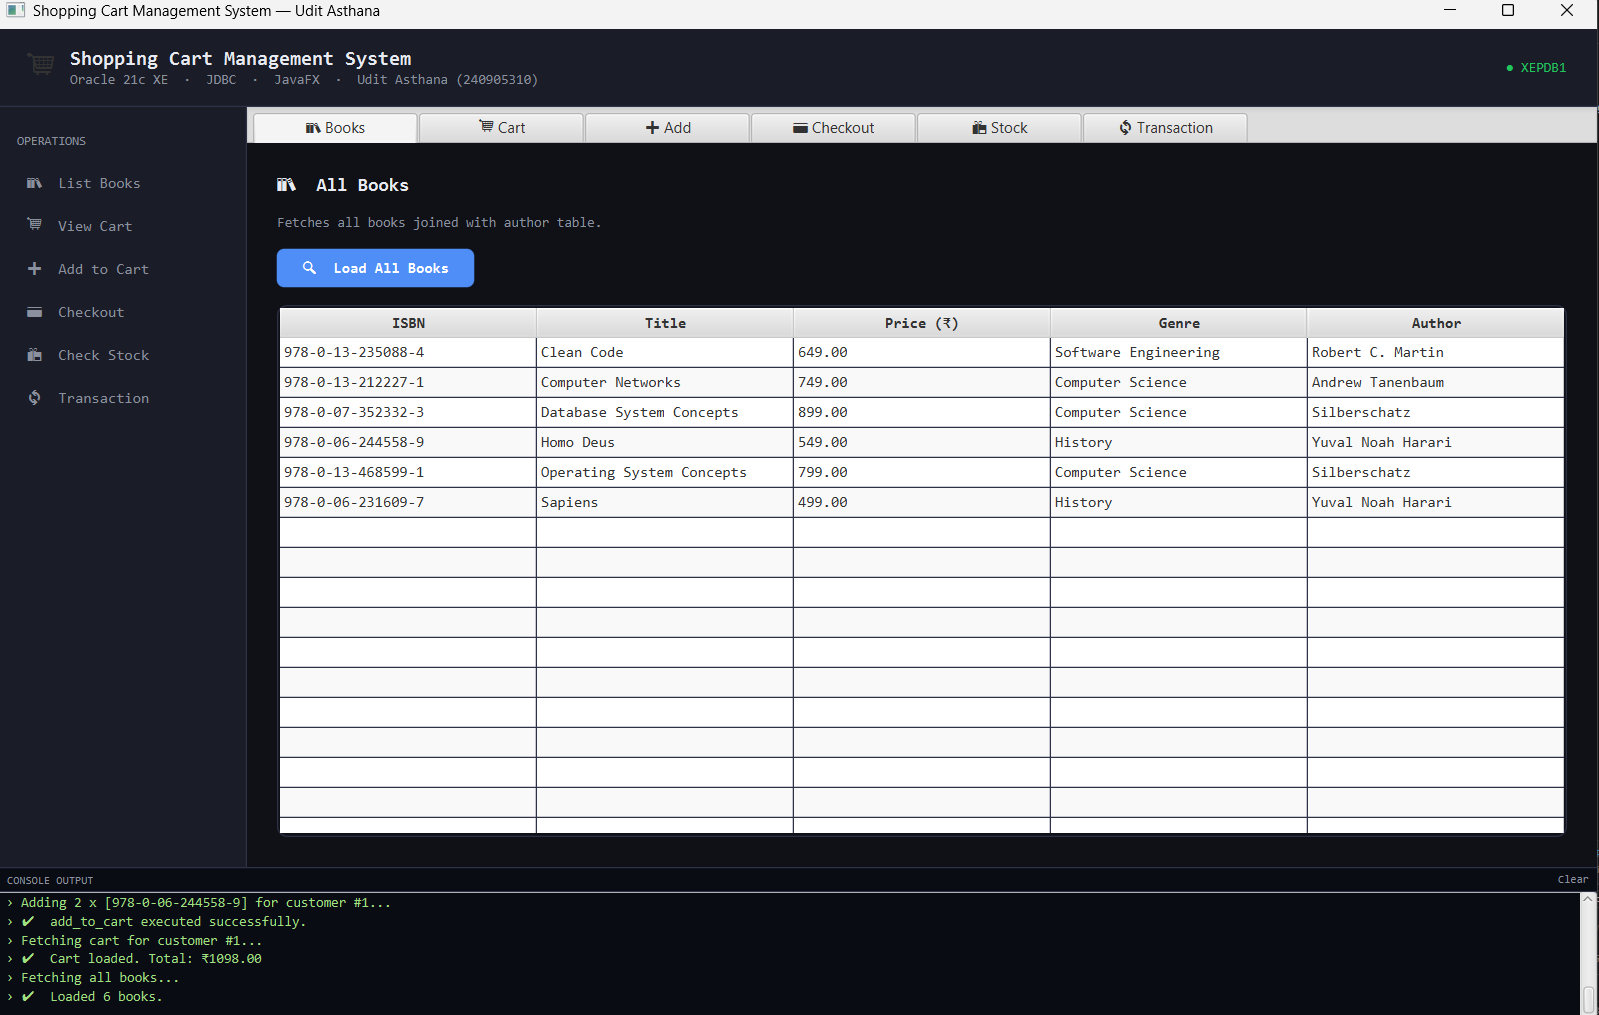
\includegraphics[width=0.92\linewidth]{ss_books.png}
    \caption{Books tab — all 6 books fetched via \texttt{SELECT ... JOIN AUTHOR}.
             Console shows \texttt{Loaded 6 books.}}
    \label{fig:ui-books}
\end{figure}

\subsection{View Cart}

\begin{figure}[H]
    \centering
    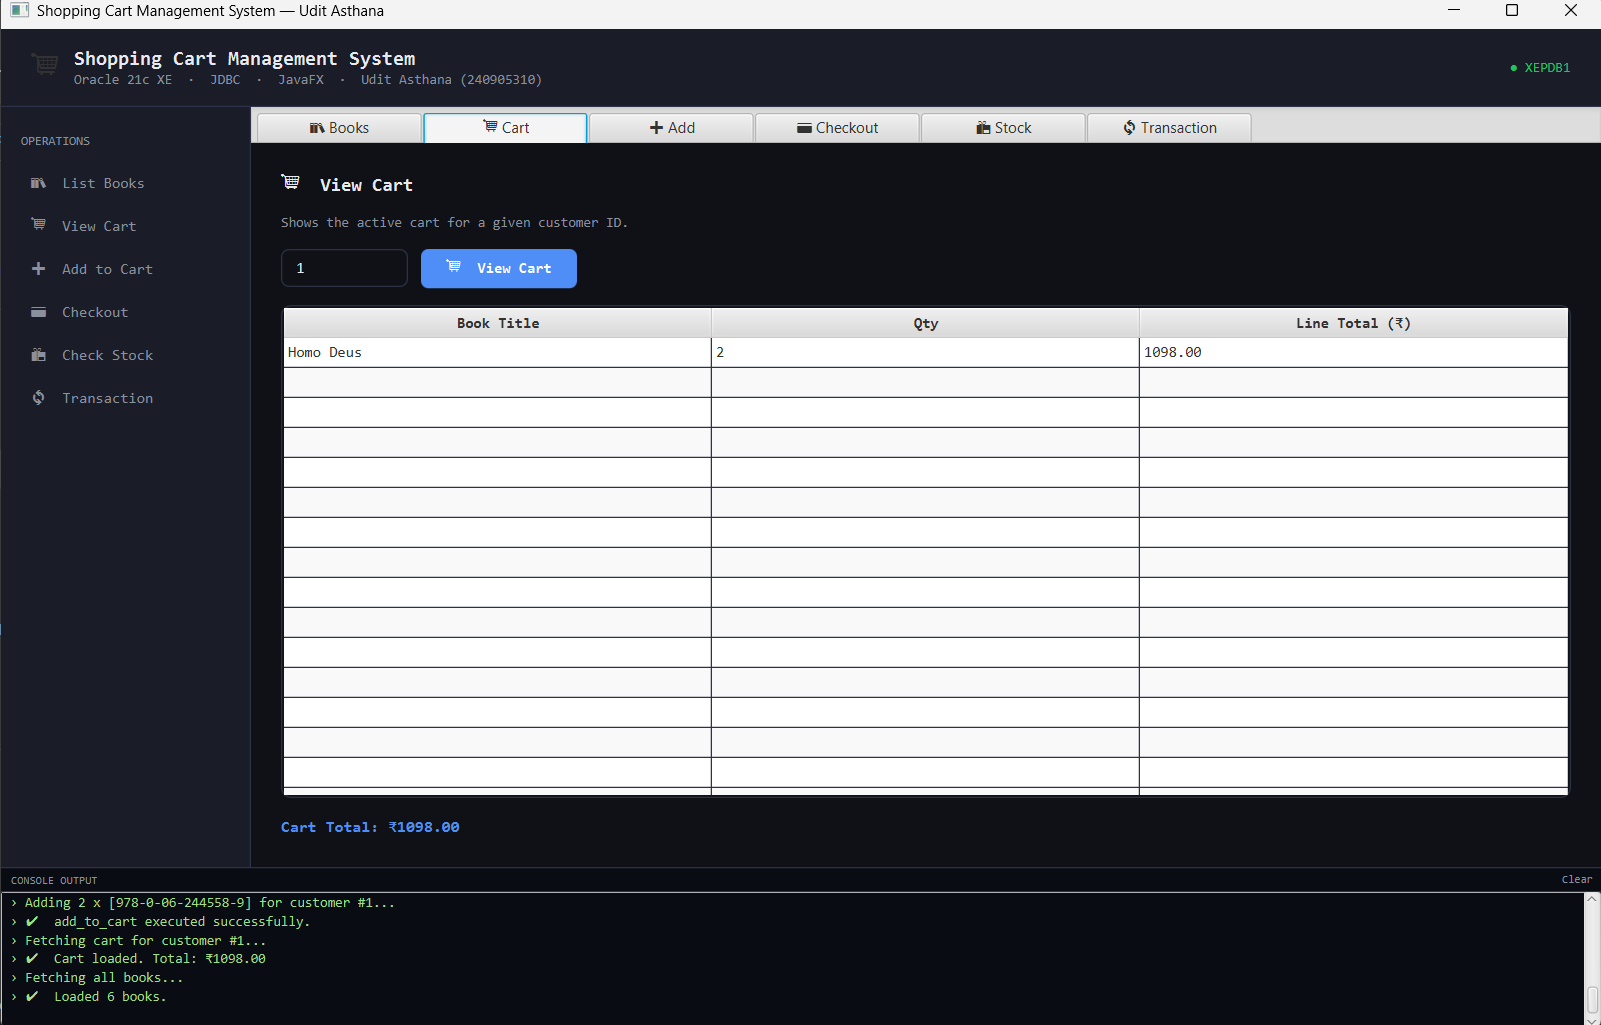
\includegraphics[width=0.92\linewidth]{ss_viewCart.png}
    \caption{Cart tab — active cart for Customer \#1 showing \textit{Homo Deus}
             (qty 2, line total ₹1098.00). Uses \texttt{PreparedStatement} with
             customer ID as parameter.}
    \label{fig:ui-cart}
\end{figure}

\subsection{Add to Cart}

\begin{figure}[H]
    \centering
    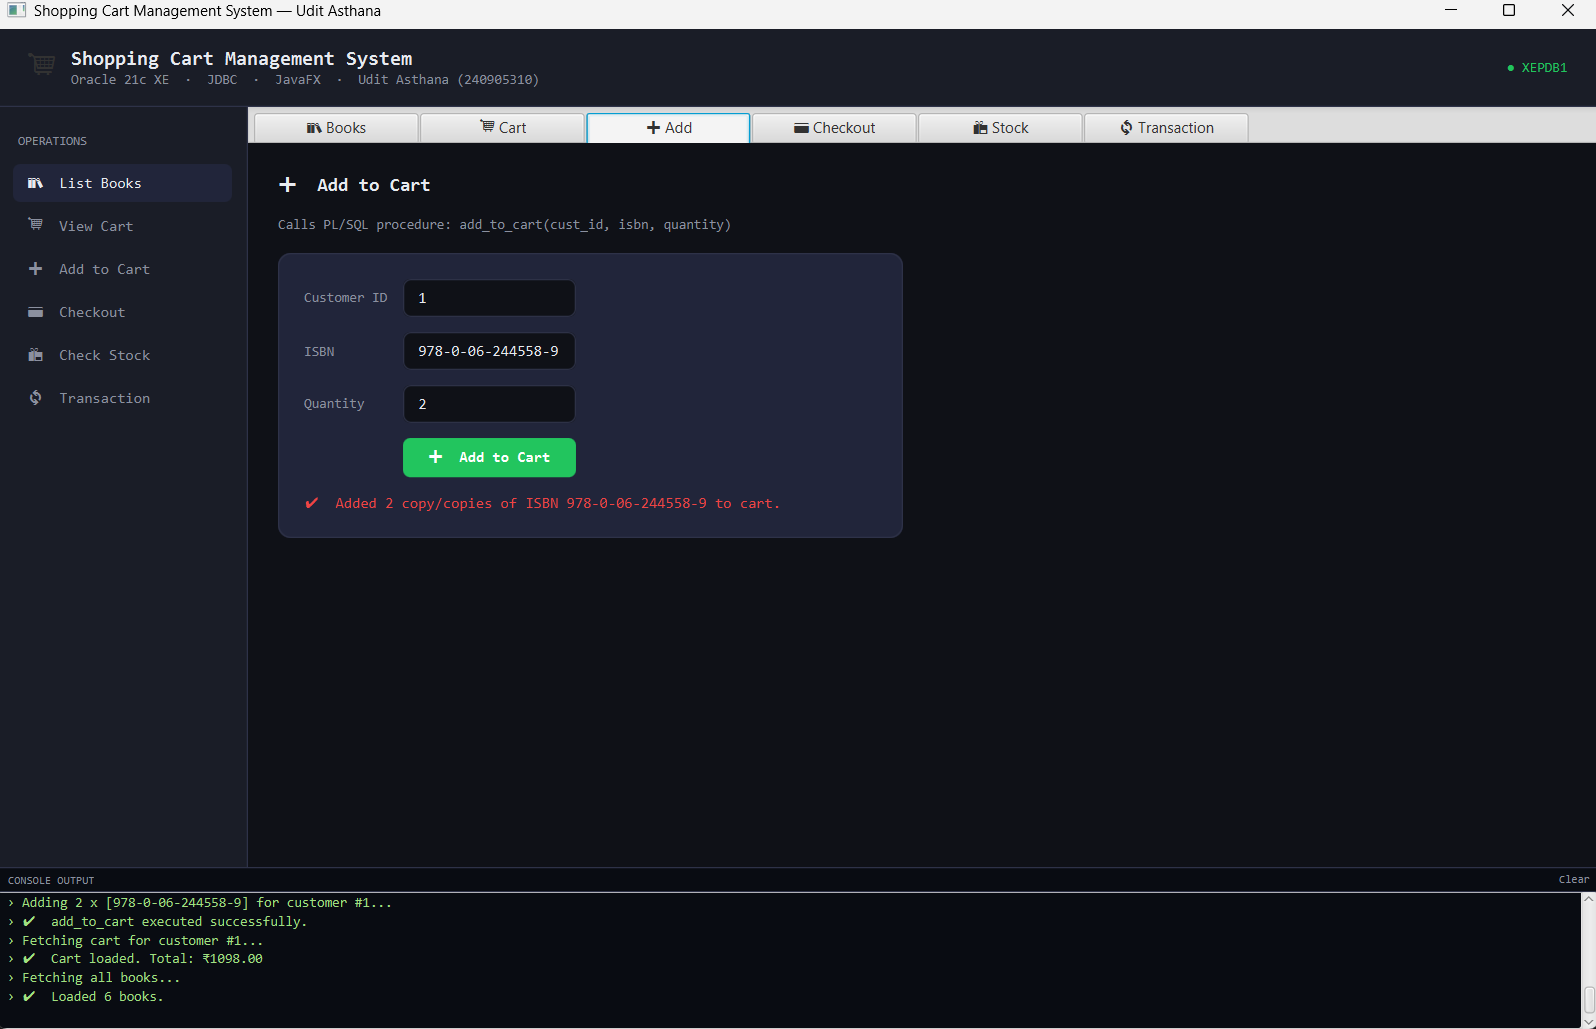
\includegraphics[width=0.92\linewidth]{ss_addToCart.png}
    \caption{Add to Cart tab — Customer \#1 adds 2 copies of ISBN
             \texttt{978-0-06-244558-9}. Calls PL/SQL procedure
             \texttt{add\_to\_cart(cust\_id, isbn, quantity)} via
             \texttt{CallableStatement}.}
    \label{fig:ui-add}
\end{figure}

\subsection{Checkout}

\begin{figure}[H]
    \centering
    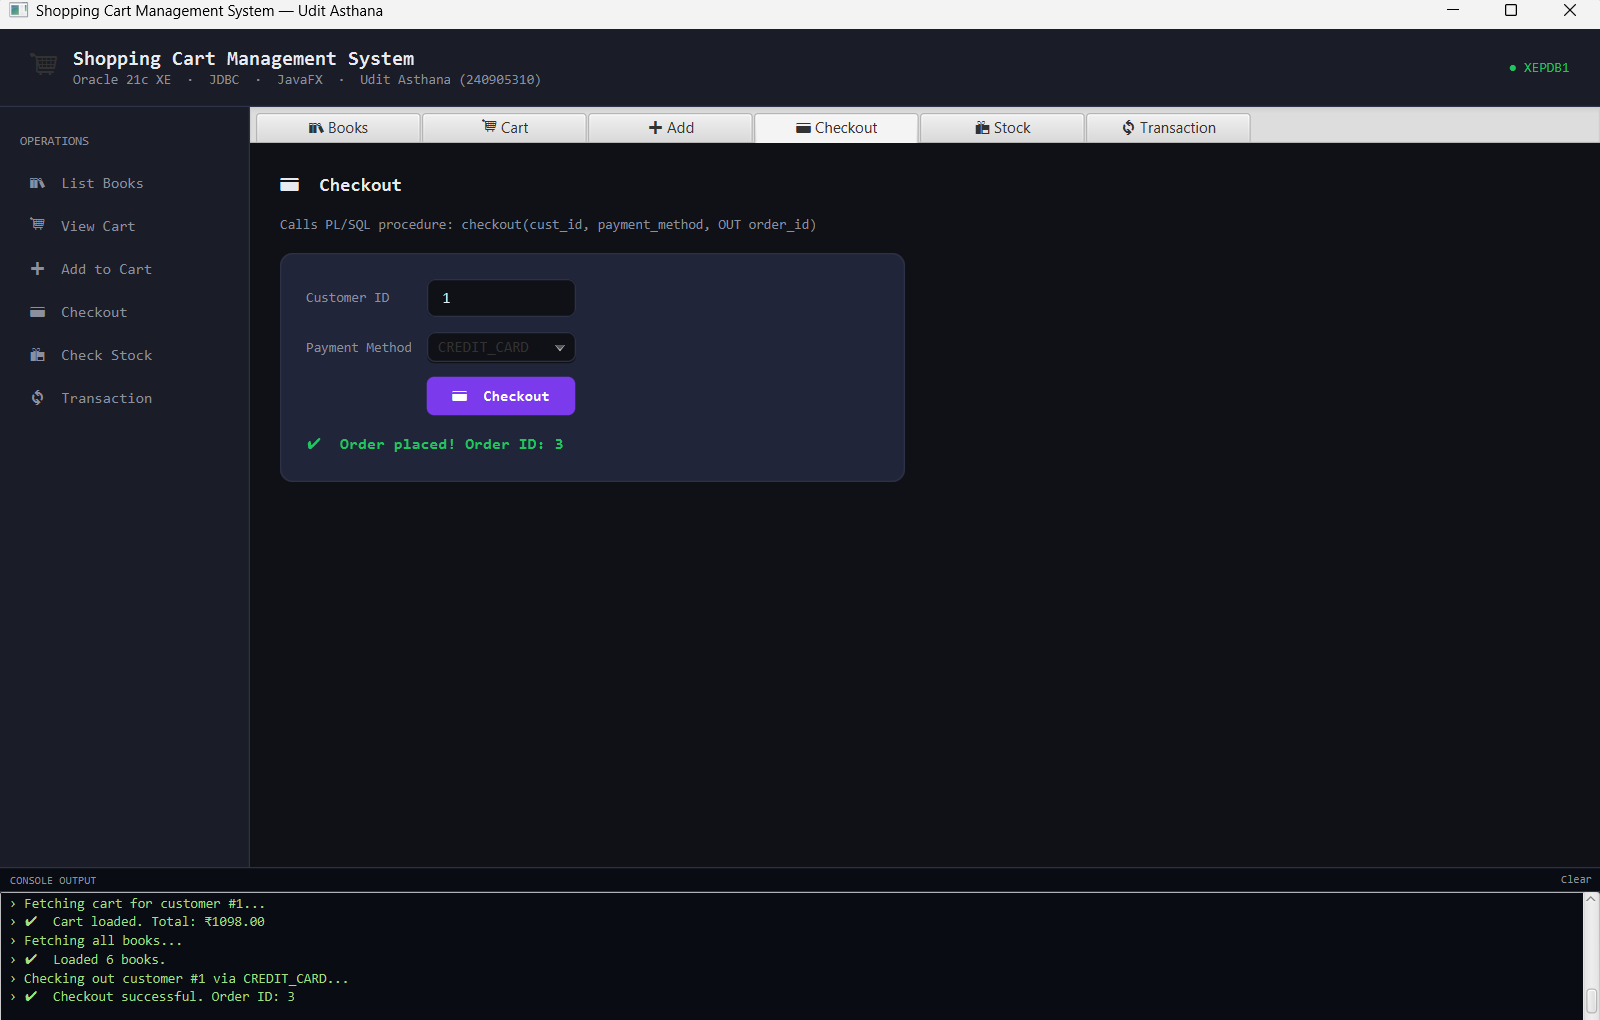
\includegraphics[width=0.92\linewidth]{ss_transaction.png}
    \caption{Checkout tab — Customer \#1 checks out via \texttt{CREDIT\_CARD}.
             Order ID 3 returned from the \texttt{checkout} PL/SQL procedure
             OUT parameter. Console confirms \texttt{Checkout successful.}}
    \label{fig:ui-checkout}
\end{figure}

\subsection{Check Stock}

\begin{figure}[H]
    \centering
    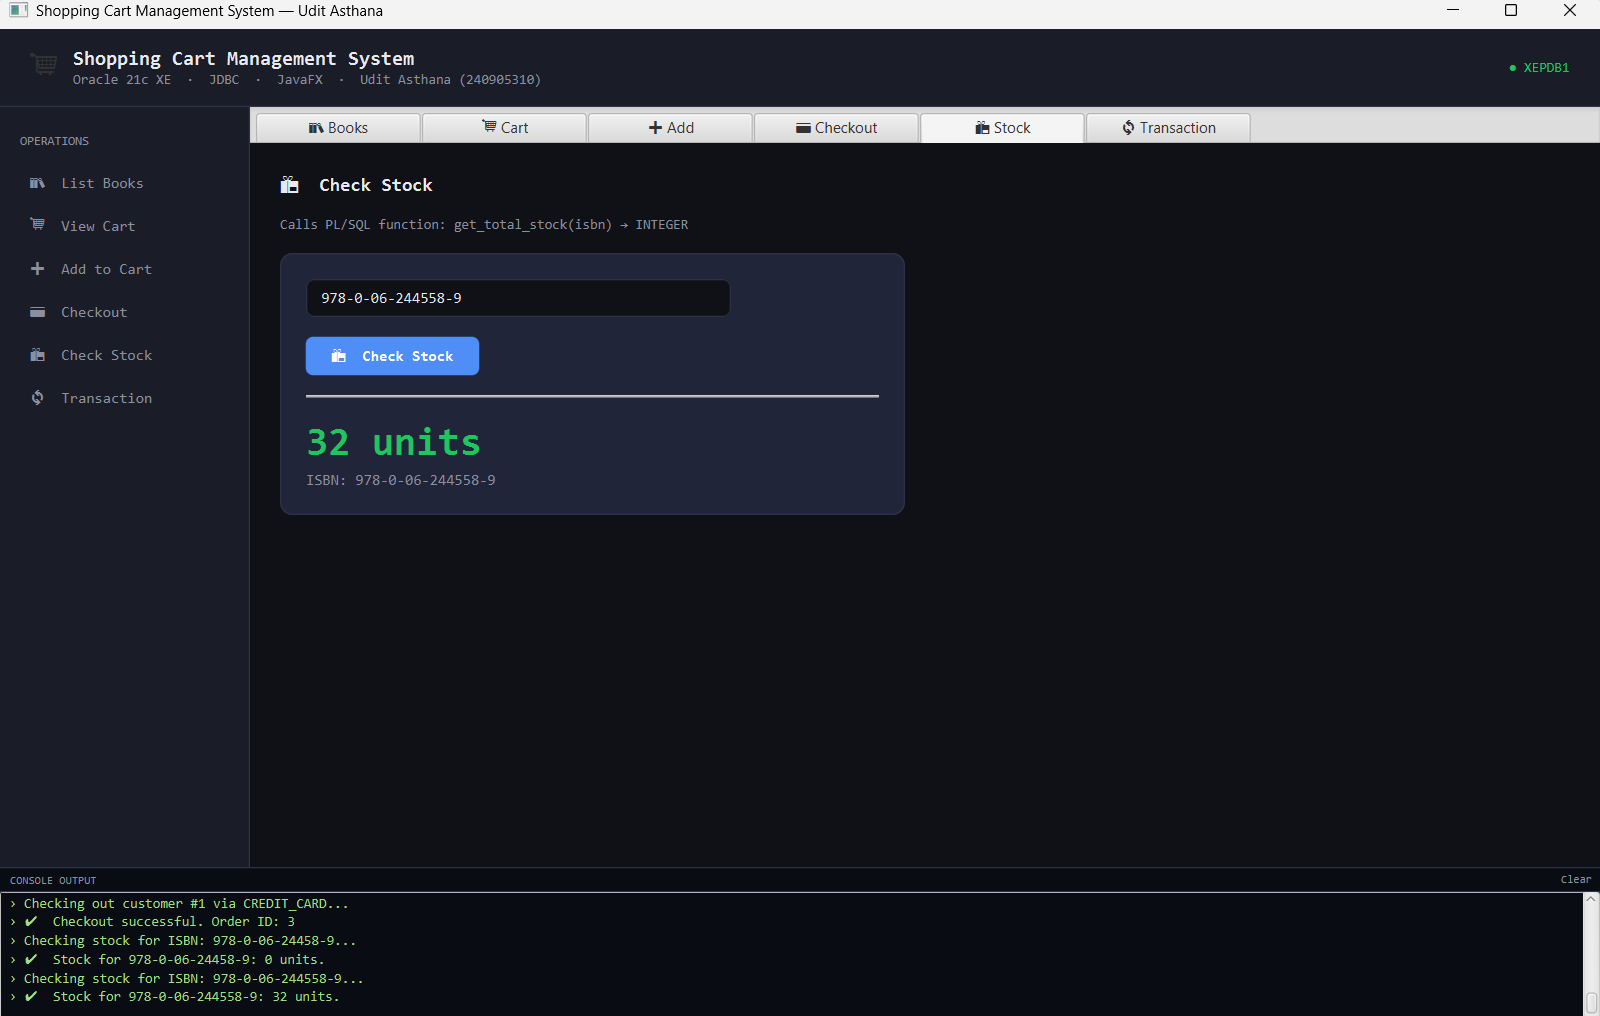
\includegraphics[width=0.92\linewidth]{ss_stock.png}
    \caption{Stock tab — calls PL/SQL function \texttt{get\_total\_stock(isbn)}
             and displays result. ISBN \texttt{978-0-06-244558-9} shows 32 units
             remaining after the checkout above decremented inventory via trigger.}
    \label{fig:ui-stock}
\end{figure}

\subsection{Transaction Demo}

\begin{figure}[H]
    \centering
    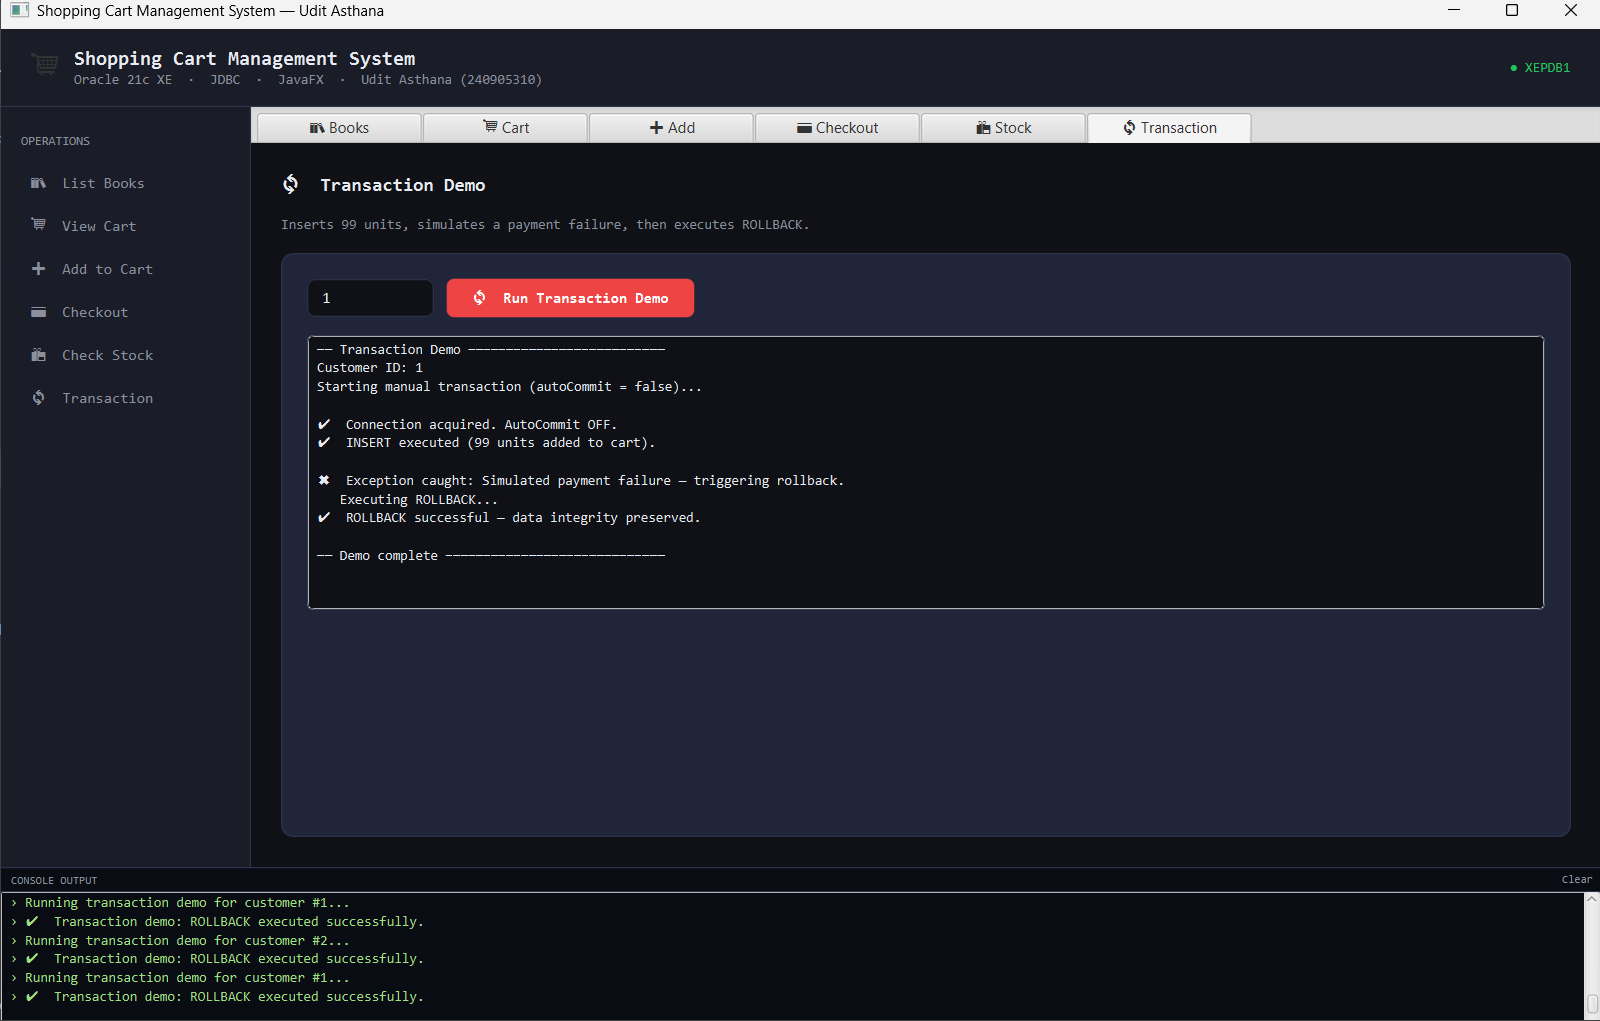
\includegraphics[width=0.92\linewidth]{ss_transactionDemo.png}
    \caption{Transaction Demo tab — inserts 99 units into cart, simulates a
             payment failure, then executes \texttt{ROLLBACK}. Demonstrates
             \texttt{con.setAutoCommit(false)} with explicit rollback on
             exception. Data integrity is preserved.}
    \label{fig:ui-transaction}
\end{figure}


\section{Testing Scenarios}


\begin{table}[H]
\centering
\caption{Test cases and expected outcomes}
\begin{tabular}{lll}
\toprule
\textbf{Test Case} & \textbf{Input} & \textbf{Expected Result} \\
\midrule
Add to cart (valid)          & ISBN + qty in stock    & Item added, cart updated \\
Add to cart (out of stock)   & qty $>$ total stock    & ORA-20010 raised \\
Checkout (valid)             & Active cart, items available & Order placed, stock decremented \\
Checkout (empty cart)        & Cart with 0 items      & ORA-20030 raised \\
Checkout (partial stock)     & One item insufficient  & ORA-20031 raised, rollback \\
Modify checked-out cart      & DML on cart\_id=2      & ORA-20060 raised (trigger) \\
Negative stock update        & SET quantity = -1      & ORA-20050 raised (trigger) \\
Duplicate email registration & Same email twice       & ORA-00001 (unique constraint) \\
\bottomrule
\end{tabular}
\end{table}


\section{Conclusion}

This project successfully demonstrates the design and implementation of a Shopping
Cart Management System grounded in rigorous DBMS principles. Starting from the
Exercise 6.21 bookstore E-R schema, the system was extended to support a complete
purchase lifecycle — from cart creation through checkout to payment recording.

Key outcomes achieved:
\begin{itemize}
    \item A fully normalised (3NF) relational schema with 11 tables.
    \item 15 SQL queries spanning basic retrieval to complex multi-table aggregation.
    \item 4 PL/SQL stored procedures and 2 functions encapsulating core business logic.
    \item 5 triggers enforcing referential and business-rule integrity automatically.
    \item An atomic, rollback-safe checkout transaction preventing partial order anomalies.
    \item A Java JDBC layer demonstrating \texttt{PreparedStatement},
          \texttt{CallableStatement}, and manual transaction control.
\end{itemize}

\subsection{Limitations}
\begin{itemize}
    \item The system supports a single active cart per customer; concurrent
          sessions are not handled.
    \item Authentication is not implemented in the UI; customer ID is entered
          manually.
    \item The JavaFX frontend is desktop-only and not suitable for web
          or mobile deployment.
    \item Inventory is decremented by trigger at order insertion but is not
          reserved during cart session, allowing race conditions under
          concurrent load.
\end{itemize}

\subsection{Future Work}
\begin{itemize}
    \item Implement session-based authentication with hashed password
          verification.
    \item Add optimistic locking or inventory reservation during cart
          checkout to handle concurrent users.
    \item Migrate the frontend to a REST API backend with a web interface.
    \item Extend reporting queries into a live analytics dashboard within
          the UI.
\end{itemize}
\section*{References}

\addcontentsline{toc}{section}{References}

\begin{enumerate}
    \item Silberschatz, A., Korth, H.F., Sudarshan, S. (2019). \textit{Database System
          Concepts}, 7th edition. McGraw-Hill.
    \item Oracle Corporation. (2021). \textit{Oracle Database 21c SQL Language Reference}.
          \url{https://docs.oracle.com/en/database/oracle/oracle-database/21/}
    \item Oracle Corporation. (2021). \textit{Oracle Database PL/SQL Language Reference}.
    \item Oracle Corporation. (2021). \textit{JDBC Developer's Guide}.
\end{enumerate}

\end{document}